% !TeX root =./main.tex
% !TeX spellcheck = en_US

Due to a global economic expansion, the transport sector has been gaining massive momentum for years.
Since 2010, global freight volumes continuously increase with forecasts predicting growth rates of 3.2\% per year until 2050 \cite{figura2020preferences, InternationalTransportForum}.
Various transportation modes, including rail, maritime, air, and road, are available to cope with this rapid development and to satisfy future transportation needs.
However, primary focus is generally placed on the road transport segment due to its dominating role for domestic transportation, with almost 80\% of the total volume of goods being carried by trucks in the European Union \cite{Eurostat}.
The increase in demand for transportation also holds true for superheavy, bulky and extra-large goods \cite{gavrilova2021analysis}, referred to as oversized and heavyweight cargoes (OHC) in this article \cite{Luo.2021}.
OHC is typically associated with the transportation of industry goods (e.g., generators, turbines, construction equipment) that exceed defined limits in terms of weight and/or size, many of which without permission, i.e, illegally \cite{fiorillo2016minimizing}. This is especially the case for cross-border activities where operators are frequently faced with different legal requirements. 
\par In comparison with traditional freight transportation, OHC requires time-consuming and complex efforts with regard to planning, approval, and execution, as no two OHC transports are completely the same \cite{Wolnowska.2019}.
Some OHC transports may require complete road closures or detours and escort by police and other law enforcement.
Consequently, planning is usually conducted on an individual level, taking the respective specifications of each OHC transport into consideration \cite{Bazaras.2013}.
In doing so, several relevant technical, administrative, and organizational criteria are subject of detailed analysis to reduce economic, social, and political risks, thereby increasing the safety of OHC transports \cite{Palsaitis.2012}.
Granular planning is further dependent on national standards and legislation. Due to legal requirements, it generally involves the evaluation of multiple factors related to restrictions in terms of roads' physical characteristics, such as road turning radius, widths, and lengths, obstacles along the road or demand for installation of transshipment sites \cite{PETRASKA.2018}.
Oversize load is particularly limited by road turning radius, transport corridor width, and road-side obstacles, such as traffic lights or power lines.
Hence, planning is dominated by local characteristics and in-person inspection is required once a particular transport route has been submitted to the authority.
Overweight load, i.e., vehicles loaded with more than 11 tons per axle, is even more difficult to plan than oversize load.
One of the most safety-relevant attributes that needs to be considered in this respect is the maximum bridge carrying capacity, which must not be surpassed by the total weight of a OHC transport, and thus, is highly influencing route planning activity.
This is for two reasons; excessive overload significantly contributes to shorten service lifes of pavements and bridges; and reduces bridge safety to levels that may fall below those set in the design standards, potentially resulting in failures or collapse \cite{fiorillo2018fragility, yan2018optimal, ghosn2000development}.
Critical incidents, such as the Genova bridge collapse in 2018 \cite{Morgese.2020, MorandiNYTimes},  demonstrate the effects of long-term exceeding of permitted limits on infrastructure, thereby underlining the importance of complying with certain standards and norms in OHC planning. However, a cornerstone for ensuring compliance is monitoring via fixed or mobile truck weighing stations \cite{fiorillo2016minimizing}.
\par In practice, the route planning process for oversize and heavyweight transports involves several stakeholders, such as client companies, carriers, governmental institutions, and civil engineers.
This labor intense planning procedure is described in \cite{Osegueda.1999}. In the beginning, the client company or carrier drafts a first route design and submits this draft to the responsible authority for approval.
Subsequently, a civil engineer is consulted to determine the maximum allowable weight and speed on every single bridge of the proposed route.
Aside from statical calculations, the civil engineer relies on on-site visits and inspections of bridge elements to evaluate their tolerances, technical specifications, and other structural parameters.
In case of route infeasibility due to exceeding of permitted limits or for any other reason, the initial draft needs to be revised, adapted, and resubmitted by the applicant and subsequently re-evaluated by the civil engineer.
This costly and time-consuming process must be repeated until the route is declared feasible and a permit is granted. As of this moment, the approved route must not be deviated from.
What seems to be problematic in this respect is that the development of the initial draft is primarily based on commercial GIS applications that are limited in terms of data availability and accuracy.
Standard GIS solutions indeed consider temporary construction sites or road closures but exhibit a severe lack of data on bridge locations and the respective carrying capacities, and thus, do not facilitate the identification of an optimal route under consideration of weight limits.
Therefore, there is a need of professional software that thoroughly takes weight parameters into account.
\par In an attempt to simplify the cumbersome authorization process, we take an optimization approach.
To this end, a mathematical model is used to determine the optimal path between two points within the road network while respecting certain constraints, i.e., weight limits, for example.
Under the assumption that the model results in more than one feasible routes, a study that compares several (possibly conflicting) objectives will be conducted.
In doing so, we consider different types of vehicles and loads. The results should provide \textit{decision support} for reducing the complexity of OHC route planning. 
\par
The article continues in section 2 with a review of the existing body of knowledge in the respective field.
In section 3, we provide the problem description and introduce notations along with the model assumptions. In section 4, the optimization model is presented and illustrated in an example of application.
Finally, section 5 closes the article, summarizing the research implications, study limitations, and future lines of research.



\begin{figure}[!ht]
  \centering
  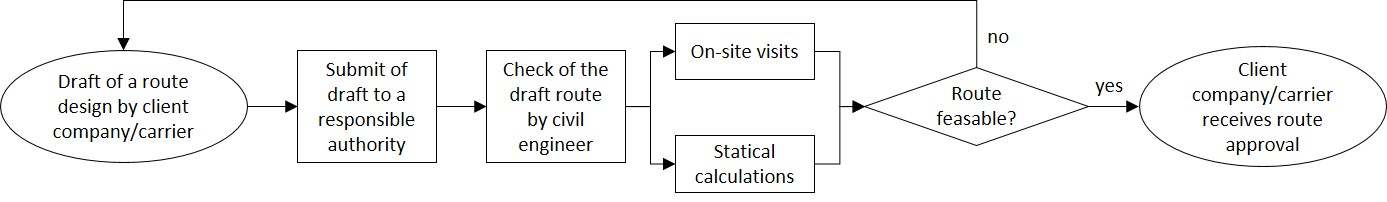
\includegraphics[width=0.9\textwidth]{OHCfinal.jpg}
  \caption{Overview of the higher level road network in Carinthia.}
  \label{fig:higher level}
\end{figure}
